\chapter{Optimization Strategies}
\label{ch:optimization}

The following chapter will present optimization strategies which were used to
accelerate the mean shift image segmentation. The presented strategies are not
only valid for \gls{CUDA}, they can be applied to many parallel machines which
are build after the shared memory or \gls{SPMD} model. The chapter is divided in
several sections. Each section will present an optimization. The are major and
minor optimization that are examined where mostly major optimization give higher
speedup whereas minor optimization give lower speedup. 

Many of the optimization are hardware centric, which means that one has to have
a good knowledge about the architecture to understand which steps can be
undertaken to accelerate the algorithm and which where even possible. Each
section will cover the architectural specialty which led to perform the specific
optimization. The first optimization of the next section is a general rule when
trying to accelerate an algorithm, offload compute intensive parts. The succeeding
sections respectively optimizations are in chronological order and where applied
in that order, identifiable by the ever increasing speedups. 


\section{Offload Compute Intensive Parts}
\label{sec:offload_intensive}
\fpAdd{\timegold}{0,0}{11310}
\fpAdd{\timecuda}{0,0}{1942}
\fpDiv{\speedup}{11310}{1942}

As shown in \autoref{ch:algorithm_analysis} {\color{red} DESIGN IMPLEMNtAtION..}
the most compute intensive part of the mean shift segmentation is the filtering
step. bla bla blbub.. mal sehen was vorne noch steht 98\%. In this case the most
compute intensive part is 98.2\% of the complete run-time and hence a valuable
part to offload. All other parts have no significant part of the run-time but
when optimizing it can happen that these other part grow in terms of run-time
and the before most compute intensive part with a very high percentage drops to
a low percentage and hence the percentages of all other parts increase and
become very compute intensive. 

In other cases the run-time is often distributed among several parts and in this
case it should be tried to offload as much as possible of the computational parts
to an accelerator as the \gls{GPU}. In the first place the focus will be on the
filter part that is executing in total 99.1\% of the run-time.

For the following considerations about speedup the \autoref{eq:speedup} will be
used to calculate the speedup. 

In {\color{red} bezug zu design implementierun} it was shown how to design and
to implement the algorithm to offload the important parts to the \gls{GPU} and
the first naive implementation of the mean shift filter in \gls{CUDA} resulted
in a speedup of

\begin{equation*}\label{eq:speedup0}
	S = \frac{T_{CPU}}{T_{GPU}} = %
	\frac{\unit[\timegold]{ms}}{\unit[\timecuda]{ms}} = \speedup
\end{equation*}

times faster than the \gls{CPU} version. The reference time was generated from
\href{http://www.caip.rutgers.edu/riul/research/code.html}{ \gls{EDISON}}. It
reports timings for filtering and segmentation.
 The naive implementation was 

\section*{Optimize Access to Global Memory}
\label{sec:coalescing}

One important fact for coalescing is the sequential accesses to global memory
should be grouped together. A simple optimization is to use the \emph{float4}
data type available in \gls{CUDA}. After rewriting the algorithm the new speedup
was 
\fpAdd{\timecuda}{0,0}{1464}
\fpDiv{\speedup}{\timegold}{\timecuda}
\begin{equation*}\label{eq:speedup0}
	S = \timegold\ ms/\timecuda\ ms = \speedup
\end{equation*}

basin of attraction, random access to global memory, not knowing where each pixel
is moving to. Switching to \emph{textures} (glossary texturess) yield to a huge
speedup of 

\fpAdd{\timecuda}{0,0}{260}
\fpDiv{\speedup}{\timegold}{\timecuda}
\begin{equation*}\label{eq:speedup0}
	S = \timegold\ ms/\timecuda\ ms = \speedup
\end{equation*}


\section*{Avoid Expensive Divisions}
\label{sec:expensive_divisions}

If possible precalculate divisions. For example if it looks like this
\begin{lstlisting}[caption=Divison, label=lst:division]
dl = (luv.x - yj_2) / sigmaR;               
du = (luv.y - yj_3) / sigmaR;               
dv = (luv.z - yj_4) / sigmaR;
\end{lstlisting}
one can calculate \emph{rsigmaR = 1.0f/sigma} in advance and everywhere where a division by
$sigmaR$ occurs replace it into a multiplication. The resulting code is
\begin{lstlisting}[caption=Precalculated Divison, label=lst:precalcdivision]
dl = (luv.x - yj_2) * rsigmaR;               
du = (luv.y - yj_3) * rsigmaR;               
dv = (luv.z - yj_4) * rsigmaR;
\end{lstlisting}

This optimization yielded  a speedup of 

\fpAdd{\timecuda}{0,0}{203}
\fpDiv{\speedup}{\timegold}{\timecuda}
\begin{equation*}\label{eq:speedup0}
	S = \timegold\ ms/\timecuda\ ms = \speedup
\end{equation*}


\section{Run Configurations} % (fold)
\label{sec:run_configurations}

It is important to check the best run configuration. Each run configruation 
has its benefit. Some can exploit the bandwidth to the global memory some can
benefit from the cache of the texture. After testing all configurations the 
best fit was a $8x32=256 threads$ configuration.

\fpAdd{\timecuda}{0,0}{181}
\fpDiv{\speedup}{\timegold}{\timecuda}
\begin{equation*}\label{eq:speedup0}
	S = \timegold\ ms/\timecuda\ ms = \speedup
\end{equation*}


% section run_configurations (end)

\section{Use the Float Data Type where Ever Possible}
One should use the $float$ data type where ever possible. \glspl{GPU} are 
highly optimized for floating point calculations. After converting all integer
calculations to floating point operations another significant speedup was 
achieved.
\fpAdd{\timecuda}{0,0}{175}
\fpDiv{\speedup}{\timegold}{\timecuda}
\begin{equation*}\label{eq:speedup0}
	S = \timegold\ ms/\timecuda\ ms = \speedup
\end{equation*}


\section{Avoid Branch Divergence} % (fold)
\label{sec:avoid_branch_divergence}
On a architecture with such high throughput of calculations per cycle it is preferred
to calculate values rather then generating them through $if$ and $else$ statements.
The remaining $if$ and $else$ statements where arranged in such a way so that a 
thread is exiting early from the loop and avoiding uneccesary calculations. This leads
of course to higher branch divergence but the execution time is lower. 
\fpAdd{\timecuda}{0,0}{125}
\fpDiv{\speedup}{\timegold}{\timecuda}
\begin{equation*}\label{eq:speedup0}
	S = \timegold\ ms/\timecuda\ ms = \speedup
\end{equation*}

\section{Shared Memory} % (fold)
\label{sec:shared_memory}
The optimization guides state that one should use shared memory to avoid 
redundant transfers from global memory. But in this case the accesses are not 
known in advance and would lead to heavy reduce in run time as the access to 
shared memory from the threads would lead to many bank conflicts. 

\section{Know the Algorithm} % (fold)
\label{sec:know_the_algo}

experiments to know how many iterations are used per pixel.... 
variying the $limit$
Setting the $lim = 10$ and executing the \gls{CPU} and \gls{GPU} version we get
\fpAdd{\tgold}{0}{7369}
\fpAdd{\tcuda}{0}{29}
\fpDiv{\speedup}{\tgold}{\tcuda}
\begin{equation*}\label{eq:speedup0}
	S = \timegold\ ms/\timecuda\ ms = \speedup
\end{equation*}


Setting the $lim = 50$ and executing the \gls{CPU} and \gls{GPU} version we get
\fpAdd{\tgold}{0}{10373}
\fpAdd{\tcuda}{0}{82}
\fpDiv{\speedup}{\tgold}{\tcuda}
\begin{equation*}\label{eq:speedup0}
	S = \timegold\ ms/\timecuda\ ms = \speedup
\end{equation*}


\begin{figure}[ht]
\centering
\subfloat[Period-0 Limitcycle]{%
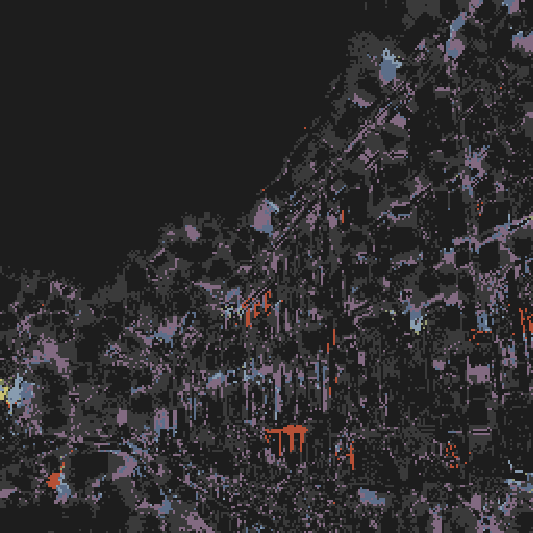
\includegraphics[width=0.33\textwidth]{gfx/itr_limitcycle0}\label{fig:lc0}}%
\subfloat[Period-4 Limitcycle]{%
\includegraphics[width=0.33\textwidth]{gfx/itr_limitcycle4}\label{fig:lc4}}%
\subfloat[Period-8 Limitcycle]{%
\includegraphics[width=0.33\textwidth]{gfx/itr_limitcycle8}\label{fig:lc8}}%

\caption{Effect of limitcycle detection on iteration count}
\label{fig:limitcycle}
\end{figure}


\begin{figure}[ht]
\centering
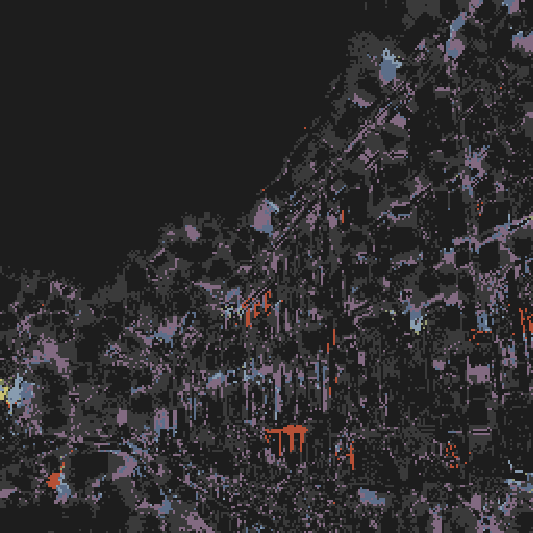
\includegraphics[width=0.6\textwidth]{gfx/itr_limitcycle0.pdf}
\caption{Visualization of Iteration Count}
\label{fig:vis_iteration_count}
\end{figure}

Looking at the iteration count  iter.txt one can see that pixel $10992$ has an 
iteration count  of $100$. 
$ i = 10992 mag=2,5 iter=100$. Examining the sequence of the magnitude one can 
easily see that after some iterations the magnitude is fixed to $2.5$. This
behaviour is known as a fixed point limit cycle.

\subsubsection{Limit Cycle, Iterating Dynamical Systems} % (fold)
\label{ssub:limit_cycle_iterating_dynamical_systems}
bla bla  limit cycle attractors...


examining $i = 15762$ shows that the iteration is a period-2 limit cycle.

Implementing a simple period-4 limit cycle detection yields to a speedup of
\fpAdd{\timecuda}{0,0}{99}
\fpDiv{\speedup}{\timegold}{\timecuda}
\begin{equation*}\label{eq:speedup0}
	S = \timegold\ ms/\timecuda\ ms = \speedup
\end{equation*}

Implementing a simple period-8 limit cycle detection yields to a speedup of
\fpAdd{\timecuda}{0,0}{87}
\fpDiv{\speedup}{\timegold}{\timecuda}
\begin{equation*}\label{eq:speedup0}
	S = \timegold\ ms/\timecuda\ ms = \speedup
\end{equation*}


\section{Unrolling Loops and Multiplications} % (fold)
\label{sec:unrolling_loops_and_multiplications}

After unrolling the multiplications 
\fpAdd{\timecuda}{0,0}{83}
\fpDiv{\speedup}{\timegold}{\timecuda}
\begin{equation*}\label{eq:speedup0}
	S = \timegold\ ms/\timecuda\ ms = \speedup
\end{equation*}

\section{Extra luv to rgb Kernel}

After a lot of optimization the most computational task became really small. Now
small function which where a tiny fraction of the complete run time became 
significant. 
After implementing a $luvtorgb$ kernel the speedup is 
\fpAdd{\timecuda}{0,0}{75}
\fpDiv{\speedup}{\timegold}{\timecuda}
\begin{equation*}\label{eq:speedup0}
	S = \timegold\ ms/\timecuda\ ms = \speedup
\end{equation*}



After a lot of optimization the most computational task became really small. Now
small function which where a tiny fraction of the complete run time became 
significant. 
After a lot of optimization the most computational task became really small. Now
small function which where a tiny fraction of the complete run time became 
significant. 
After a lot of optimization the most computational task became really small. Now
small function which where a tiny fraction of the complete run time became 
significant. 










